\documentclass[10pt,twocolumn]{article}
\usepackage[margin=0.72in]{geometry}
\usepackage{amsmath,amssymb,booktabs,graphicx,microtype}
\usepackage[dvipsnames]{xcolor}
\usepackage{hyperref}
\usepackage{url}
\usepackage{enumitem}
\usepackage{float}
\usepackage{tikz}
\usetikzlibrary{arrows.meta,positioning,fit}
\hypersetup{colorlinks=true,linkcolor=MidnightBlue,citecolor=MidnightBlue,urlcolor=MidnightBlue}
\setlist{nosep,leftmargin=*}
\graphicspath{{figures/}}
\newcommand{\TrainCases}{640}
\newcommand{\TestCases}{384}
\newcommand{\OODCases}{40}
\newcommand{\RulesFOne}{0.338}
\newcommand{\PairFOne}{0.442}
\newcommand{\NeuroFOne}{0.713}
\newcommand{\NeuroPrecision}{0.679}
\newcommand{\NeuroRecall}{0.750}
\newcommand{\RulesFalsePass}{153}
\newcommand{\NeuroFalsePass}{48}
\newcommand{\NeuroFalseBlock}{68}
\newcommand{\McNemarP}{0.0101}
\newcommand{\BootstrapLow}{0.276}
\newcommand{\BootstrapHigh}{0.473}
\newcommand{\OODCombined}{1.000}
\newcommand{\OODLearned}{0.800}
\newcommand{\PairBothCorrect}{0.422}
\newcommand{\VOneRulesFOne}{0.400}
\newcommand{\VOneTfidfFOne}{0.889}

\newcommand{\system}{\textsc{Dispute Integrity Gate}}
\newcommand{\dataset}{\textsc{DIG-FECL-SYN-v2}}
\newcommand{\pass}{\textsc{Pass}}
\newcommand{\review}{\textsc{Review}}
\newcommand{\block}{\textsc{Block}}
\title{Financial Evidence Consistency Learning under Asymmetric Risk:\\A Falsification-First Neuro-Symbolic Study}
\author{Dispute Integrity Gate Research Team\\\texttt{reproducible artifact manuscript}}
\date{September 2026}

\begin{document}
\maketitle

\begin{abstract}
Chargeback evidence automation is often framed as document classification, although the operational question is relational: does heterogeneous merchant evidence agree with authoritative payment state? We formulate Financial Evidence Consistency Learning (FECL), where learned semantics may extract a grounded claim but cannot alter money or determine ledger truth. We construct \dataset, a synthetic, provenance-marked benchmark with \TrainCases{} training cases, \TestCases{} frozen family-shifted test cases, paired counterfactuals, and \OODCases{} malformed or adversarial inputs. Nine preregistered systems span literal rules, lexical models, frozen sentence embeddings, a relation-vector classifier, a compact neuro-symbolic model, XGBoost, and a five-seed MLP ensemble. The promoted research candidate obtains test F1 \NeuroFOne{} versus \RulesFOne{} for literal rules, with an exact paired McNemar $p=\McNemarP$ and bootstrap F1 improvement interval $[\BootstrapLow,\BootstrapHigh]$. Yet it produces \NeuroFalseBlock{} false blocks, calibration worsens Brier score and ECE, and only \PairBothCorrect{} of counterfactual pairs are jointly correct. We therefore reject learned autonomous blocking and retain deterministic financial invariants as the deployed safety boundary. A combined schema-and-distance controller rejects \OODCombined{} of the preregistered OOD set. The contribution is not a production-quality model claim: it is an auditable experimental system that makes evidence, semantic claims, deterministic reconciliation, abstention, and repair causally inspectable.
\end{abstract}

\section{Problem formulation}
A dispute case contains communication evidence $E$, authoritative payment state $S$, and a merchant assertion about a refund. The target $y\in\{0,1\}$ denotes whether the assertion is contradicted by $S$. The system must ground a semantic claim $c=g(E)$ to an exact source span, reconcile it through deterministic invariants $r(c,S)$, and either issue a provisional outcome or abstain. Crucially, $g$ is learned while $S$ and the money comparisons are not.

For a decision rule $d$, false PASS is materially more costly than false BLOCK in the illustrative, preregistered loss:
\begin{align}
 \mathcal{L}(d,y)={}&10\,\mathbf{1}[d=\pass,y=1]
 +\mathbf{1}[d=\block,y=0]\nonumber\\
 &+0.25\,\mathbf{1}[d=\review].
\end{align}
These weights are sensitivity-analysis parameters, not measured Razorpay economics. Precision, recall, PR-AUC, calibration, loss, latency, and risk--coverage must therefore be reported together.

\section{Merchant failure and scope}
The scoped loss is a refund-not-processed dispute in which prose can say ``refunded'' while the authoritative refund ledger is absent, incomplete, or inconsistent. Real evidence submission requires transaction-specific documents and fields \cite{razorpay2026disputes}; our system verifies a prepared evidence package before submission. It is defense-only, read-only, and cannot refund, accept liability, contact a customer, or submit evidence. The user-visible loop is
\begin{multline*}
E\rightarrow c\rightarrow r(c,S)\rightarrow\\
\{\pass,\review,\block\}\rightarrow E'\rightarrow\Delta d.
\end{multline*}

\section{Research questions and hypotheses}
\textbf{RQ1:} Does explicit evidence--state relational representation generalize beyond literal rules and bag-of-words? \textbf{H1:} a grounded semantic-state representation improves F1 and asymmetric loss on unseen language families. \textbf{RQ2:} Do deterministic money edges matter? \textbf{H2:} removing amount and currency edges lowers F1. \textbf{RQ3:} can confidence alone safely detect malformed or adversarial evidence? \textbf{H3:} no; deterministic schema validation is necessary. \textbf{RQ4:} does post-hoc calibration improve all operational criteria? \textbf{H4:} no; calibration may trade ranking and threshold behavior against probability quality.

\section{Related work and technical whitespace}
Document-level NLI grounds entailment and contradiction in long legal evidence \cite{koreeda2021contractnli}; factual entailment studies show that semantic consistency differs from topic similarity \cite{morlan2024factual}. Sentence-BERT supplies efficient semantic representations \cite{reimers2019sbert}, but cosine similarity alone does not encode which financial state is authoritative. Fraud GNNs exploit connected events and class imbalance \cite{dou2020caregnn,liu2021pcgnn}, while xFraud emphasizes explanations over transaction graphs \cite{rao2022xfraud}. Our single-case benchmark contains neither a genuine entity graph nor image pixels, so claiming GNN or multimodal benefit would be architecture theatre.

Selective prediction \cite{geifman2019selectivenet}, energy-based OOD detection \cite{liu2020energy}, temperature scaling \cite{guo2017calibration}, and conformal risk control \cite{angelopoulos2024crc} motivate abstention. The technical whitespace examined here is narrower: semantic claims are learned and grounded, but authoritative payment reconciliation remains typed, deterministic, replayable, and outside the model.

\section{Dataset}
\dataset{} is programmatically generated from explicit templates and is not evidence of field performance. Each record stores case ID, language family, source text, grounded span coordinates, communication claim, ledger state, amount, currency, label, and paired-counterfactual ID. The generated corpus contains \TrainCases{} train, 256 development, \TestCases{} frozen test, and \OODCases{} OOD cases. Every positive has a minimally edited negative counterpart sharing non-causal surface structure.

\subsection{Leakage controls}
Template families are disjoint: training uses formal, support, portal, terse, and training-Hinglish; development uses narrative and passive; frozen test uses indirect, temporal, and held-out Hinglish. Split membership is assigned before text generation, cases are grouped by counterfactual pair, and manifest hashes bind data, runner, protocol, development output, and the once-opened test result. The test set is never read by model fitting, threshold fitting, feature vocabulary construction, or Platt calibration.

\subsection{Threats from synthetic construction}
Balanced labels, templated amounts, clean ground-truth spans, and controlled family shifts make causal evaluation possible but understate OCR noise, merchant-specific style, rare payment states, multilingual morphology, and adversarial adaptation. The dataset card labels all records synthetic. No claim here transfers directly to live Indian BFSI traffic.

\section{System architecture}
Figure~\ref{fig:architecture} separates learned and deterministic authority. An immutable case envelope enters schema and injection guards. A semantic model emits a typed claim and span pointer. Deterministic code compares amount, currency, status, timestamps, and ledger presence. An uncertainty controller may only increase caution. The policy engine creates a provisional decision; a human repairs evidence and triggers a complete replay. Every node records artifact version, input hash, output hash, and duration.

\begin{figure*}[t]
\centering
\resizebox{0.96\textwidth}{!}{%
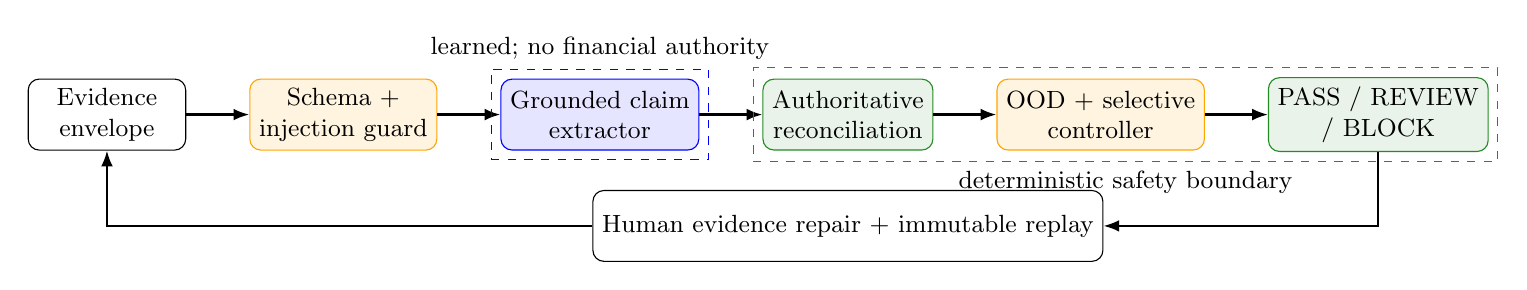
\begin{tikzpicture}[node distance=5mm and 8mm, every node/.style={font=\small}, box/.style={draw,rounded corners,align=center,minimum height=9mm,minimum width=20mm}, learned/.style={box,fill=Blue!10,draw=Blue}, det/.style={box,fill=ForestGreen!10,draw=ForestGreen}, guard/.style={box,fill=Orange!12,draw=Orange}, arr/.style={-{Latex[length=2mm]},thick}]
\node[box] (e) {Evidence\\envelope};
\node[guard,right=of e] (v) {Schema +\\injection guard};
\node[learned,right=of v] (g) {Grounded claim\\extractor};
\node[det,right=of g] (r) {Authoritative\\reconciliation};
\node[guard,right=of r] (u) {OOD + selective\\controller};
\node[det,right=of u] (d) {PASS / REVIEW\\/ BLOCK};
\node[box,below=of r] (h) {Human evidence repair + immutable replay};
\draw[arr] (e)--(v); \draw[arr] (v)--(g); \draw[arr] (g)--(r); \draw[arr] (r)--(u); \draw[arr] (u)--(d);
\draw[arr] (d.south) |- (h.east); \draw[arr] (h.west) -| (e.south);
\node[fit=(g),draw=Blue,dashed,label=above:{learned; no financial authority}] {};
\node[fit=(r)(d),draw=ForestGreen,dashed,label=below:{deterministic safety boundary}] {};
\end{tikzpicture}
}
\caption{Evidence-to-decision graph. Blue nodes infer semantics; green nodes alone evaluate authoritative payment invariants and policy. Orange nodes fail closed.}
\label{fig:architecture}
\end{figure*}

\section{Representations and models}
We compare: (1) literal relation rules; (2) communication-only TF--IDF logistic regression; (3) pair-text TF--IDF; (4) frozen MiniLM communication embeddings; and (5) a relational embedding
\begin{equation}
z=[h_E;h_S;|h_E-h_S|;h_E\odot h_S],
\end{equation}
followed by logistic regression. Model (6), the neuro-symbolic relation candidate, maps grounded semantic states to typed, auditable edges---status compatibility, amount equality, currency equality, refund reference presence, and temporal order---then learns only their combination. Model (7) removes money edges. Model (8) uses XGBoost on the same relation features. Model (9) is a five-seed MLP ensemble.

The transformer revision is pinned. Encoders are frozen: no holdout-derived representation update is possible. A constrained LLM and LoRA were specified but rejected from the executed tournament because authenticated managed training lacked repository-write capability and local memory was insufficient for a reproducible fine-tuning job. No result is imputed for unrun methods.

\section{Training and orchestration}
The executable graph is deliberately dependency-light: validate $\rightarrow$ featurize $\rightarrow$ fit $\rightarrow$ calibrate on DEV $\rightarrow$ freeze hashes $\rightarrow$ evaluate TEST once $\rightarrow$ post-hoc analysis. This has LangGraph-equivalent state semantics without adding orchestration as an experimental variable. Artifacts record configurations, versions, seeds, split hashes, metrics, predictions, and latency. The deployed runtime remains \texttt{regex-baseline-v1}; the tournament does not mutate it.

\begin{figure}[t]
\centering
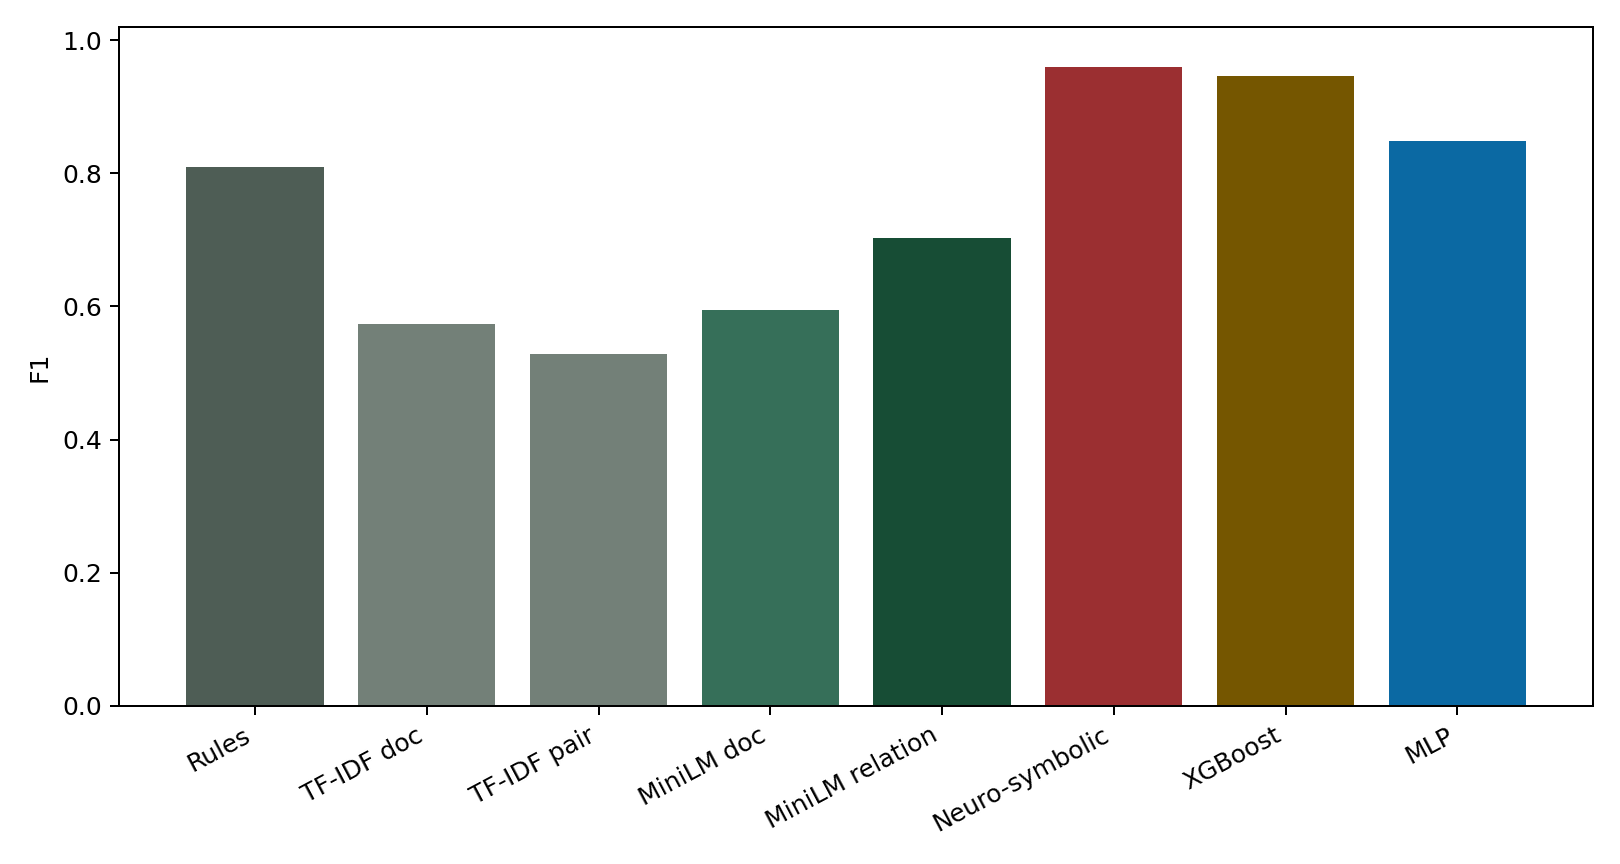
\includegraphics[width=\columnwidth]{fecl-v2-dev-f1.png}
\caption{Development F1, used for preregistered promotion decisions and calibration.}
\label{fig:devf1}
\end{figure}

\section{Evaluation protocol}
Primary model selection occurs on DEV. Before opening TEST, the protocol, runner, dataset manifest, development results, candidates, and thresholds are hashed into a freeze artifact. TEST is evaluated once. Primary endpoints are contradiction F1 and illustrative expected loss; secondary endpoints include precision, recall, PR-AUC, Brier, ECE, latency, family slices, counterfactual pair correctness, and risk--coverage. Bootstrap intervals resample paired case groups. Exact McNemar tests compare correctness vectors.

\section{Main frozen-test results}
Table~\ref{tab:main} reports DEV-fitted calibration at preregistered thresholds. Literal rules never false-block but miss \RulesFalsePass{} contradictions. The neuro-symbolic candidate raises recall from 0.203 to \NeuroRecall{} and lowers illustrative loss from 9.961 to 4.010, while introducing \NeuroFalseBlock{} false blocks. XGBoost has the lowest point estimate of illustrative loss, but it was registered as a complexity ablation, not a primary promotion candidate. We do not relabel the winner after seeing TEST.

\begin{table*}[t]
\centering\small
\begin{tabular}{lrrrrrrr}
\toprule
Model & Precision & Recall & F1 & PR-AUC & FN & FP & Cost/case\\
\midrule
Literal relation rules & 1.000 & 0.203 & 0.338 & 0.602 & 153 & 0 & 9.961 \\
Communication TF--IDF & 0.563 & 0.417 & 0.479 & 0.584 & 112 & 62 & 8.099 \\
Pair-text TF--IDF & 0.586 & 0.354 & 0.442 & 0.556 & 124 & 48 & 8.698 \\
MiniLM communication & 0.630 & 0.177 & 0.276 & 0.562 & 158 & 20 & 10.547 \\
MiniLM relation vector & 0.655 & 0.099 & 0.172 & 0.634 & 173 & 10 & 11.393 \\
Neuro-symbolic relation & 0.679 & 0.750 & 0.713 & 0.830 & 48 & 68 & 4.010 \\
Neuro-symbolic without money edges & 0.643 & 0.714 & 0.677 & 0.747 & 55 & 76 & 4.570 \\
Relation XGBoost & 0.657 & 0.818 & 0.729 & 0.647 & 35 & 82 & 3.346 \\
Relation MLP (5-seed ensemble) & 0.639 & 0.792 & 0.707 & 0.787 & 40 & 86 & 3.724 \\
\bottomrule

\end{tabular}
\caption{Frozen TEST results. ``Cost'' uses the illustrative weights in Eq. 1, not estimated merchant rupees.}
\label{tab:main}
\end{table*}

\begin{figure}[t]
\centering
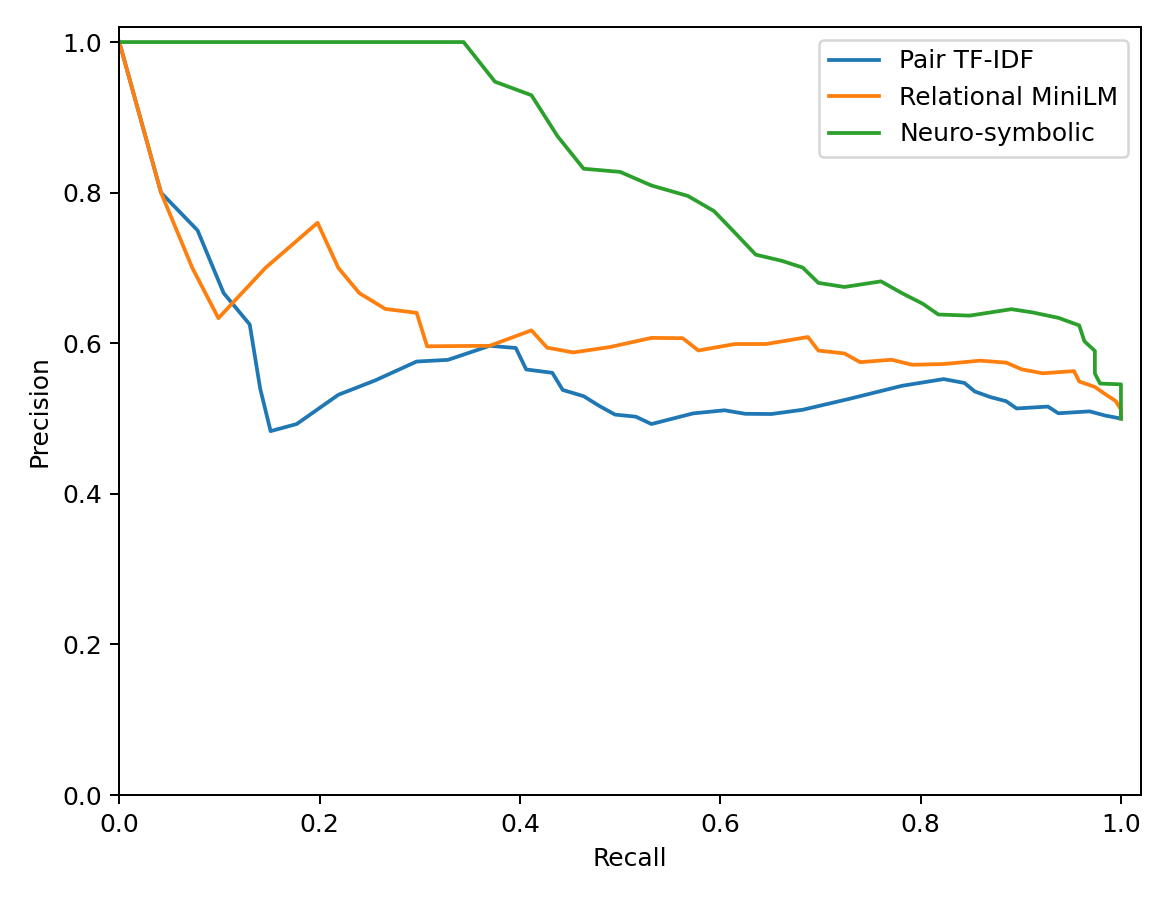
\includegraphics[width=\columnwidth]{fecl-v2-test-pr.png}
\caption{Frozen-test precision--recall curves from saved predictions.}
\label{fig:pr}
\end{figure}

\section{Statistical validation}
Against literal rules, the promoted candidate's exact paired McNemar test gives $p=\McNemarP$. A paired bootstrap over counterfactual groups estimates mean F1 lift 0.376 with 95\% interval $[\BootstrapLow,\BootstrapHigh]$. These tests reject equal casewise accuracy under this synthetic generator; they do not establish external validity or production value. Multiple exploratory comparisons are labeled secondary and are not presented as confirmatory discoveries.

\section{Ablation study}
Removing deterministic amount and currency relation edges lowers calibrated test F1 from \NeuroFOne{} to 0.677 and PR-AUC from 0.830 to 0.747. This supports H2: semantic status alone does not resolve amount and currency contradictions. Conversely, relation XGBoost only modestly exceeds the compact candidate while reducing audit simplicity. The relation-vector MiniLM model collapses after DEV-fitted calibration, showing that semantic embeddings are not automatically relational reasoning.

\section{Family and robustness slices}
\begin{table}[t]
\centering\small
\begin{tabular}{lrrrrrr}
\toprule
Family & $n$ & P & R & F1 & FN & FP\\
\midrule
hinglish\_holdout & 128 & 0.575 & 0.719 & 0.639 & 18 & 34 \\
indirect & 128 & 0.719 & 0.719 & 0.719 & 18 & 18 \\
temporal & 128 & 0.765 & 0.812 & 0.788 & 12 & 16 \\
\bottomrule

\end{tabular}
\caption{Promoted-candidate results across held-out surface families.}
\label{tab:slices}
\end{table}
Performance is weakest on held-out Hinglish (F1 0.639) and strongest on temporal language (0.788). Amount- and currency-mismatch slices reach F1 1.0, while status mismatches remain imperfect. All \NeuroFalseBlock{} false BLOCKs arise on matched controls, revealing a systematic operational harm hidden by aggregate recall.

\section{Counterfactual consistency}
Each positive/negative pair changes only the causal financial relation. Literal rules classify both members correctly for 0.203 of pairs. The neuro-symbolic model reaches only \PairBothCorrect{}, and its decision changes on 0.448 of pairs. This is clear improvement but not reliable causal invariance. The interactive lab exposes these pairs so a reviewer can edit evidence and see the finding, decision, and evidence pointer change together.

\section{Calibration}
Platt scaling is fitted on DEV only. Table~\ref{tab:cal} shows raw versus calibrated probability metrics and threshold F1 delta. Calibration is not uniformly beneficial: for the promoted model, Brier increases from 0.211 to 0.240 and ECE from 0.172 to 0.213, even though threshold F1 rises 0.014 and illustrative loss falls. Therefore the UI never displays a decorative ``confidence'' score; it displays calibration status, abstention reason, and empirical coverage risk.

\begin{table*}[t]
\centering\small
\begin{tabular}{lrrrrr}
\toprule
Model & Brier raw & Brier cal. & ECE raw & ECE cal. & $\Delta$F1\\
\midrule
MiniLM communication & 0.249 & 0.249 & 0.025 & 0.029 & -0.124 \\
Communication TF--IDF & 0.245 & 0.246 & 0.031 & 0.050 & +0.036 \\
Neuro-symbolic relation & 0.211 & 0.240 & 0.172 & 0.213 & +0.014 \\
Pair-text TF--IDF & 0.250 & 0.249 & 0.074 & 0.039 & +0.223 \\
MiniLM relation vector & 0.239 & 0.277 & 0.066 & 0.213 & -0.524 \\
Relation MLP (5-seed ensemble) & 0.204 & 0.217 & 0.112 & 0.174 & -0.004 \\
Relation XGBoost & 0.223 & 0.254 & 0.189 & 0.258 & +0.012 \\
\bottomrule

\end{tabular}
\caption{DEV-fitted calibration applied to frozen TEST. Better calibration requires lower Brier and ECE.}
\label{tab:cal}
\end{table*}

\section{Selective prediction and OOD}
For score $q_i$ and abstention threshold $\tau$, coverage and selective risk are
\begin{equation}
C(\tau)=\frac{1}{n}\sum_i\mathbf{1}[q_i\ge\tau],\quad
R(\tau)=\frac{\sum_i\ell_i\mathbf{1}[q_i\ge\tau]}{\sum_i\mathbf{1}[q_i\ge\tau]}.
\end{equation}
The learned distance/confidence detector rejects \OODLearned{} of 40 malformed, injection-like, or unsupported cases. Composing it with deterministic schema validation rejects \OODCombined{}. This supports H3 and falsifies learned-only OOD safety. The set is small and synthetic; no conformal deployment guarantee is claimed.

\begin{figure}[t]
\centering
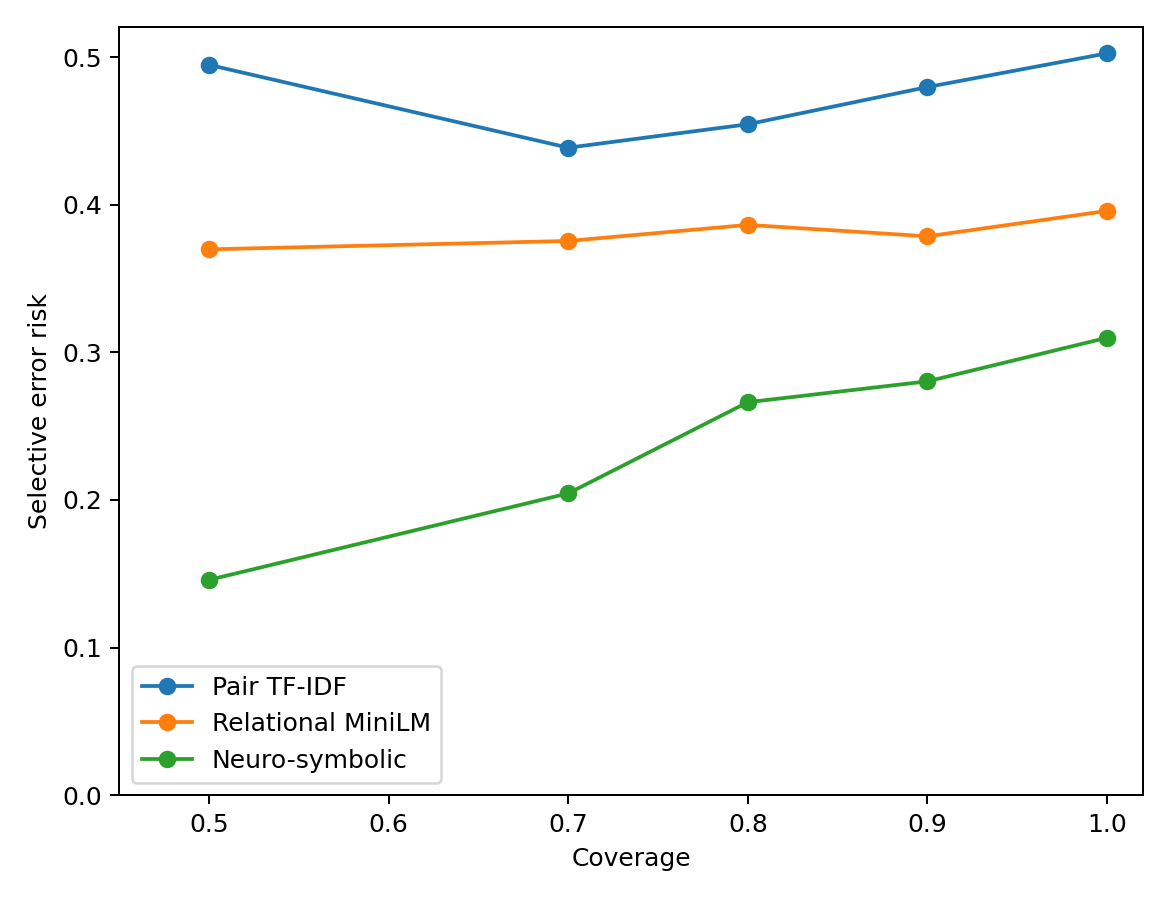
\includegraphics[width=\columnwidth]{fecl-v2-test-risk-coverage.png}
\caption{Saved frozen-test risk--coverage curves. Lower risk is preferable; declining coverage means more human review.}
\label{fig:rc}
\end{figure}

\section{Failure analysis}
False PASS examples include indirect claims such as ``the return is in flight'' when the ledger state is not processed. False BLOCK examples pair the same phrase with compatible failed or pending state. The surface cue is therefore not causal; models must resolve the direction of the communication--ledger relation. Appendix~\ref{app:errors} lists exact source excerpts and predicted probabilities. The dominant remediation is human review plus richer status semantics, not threshold tuning on TEST.

\section{Deployment decision}
The preregistered outcome is \texttt{RESEARCH\_WINNER\_NOT\_DEPLOYED}. A model can be statistically better than rules and still be unsafe for autonomous financial policy. Learned components may propose grounded spans and semantic states; deterministic invariants decide whether the ledger proves amount, currency, reference, and timing. Uncertain, malformed, unavailable, or disagreeing models route to \review. There are no autonomous financial actions.

\section{Interactive evidence debugger}
The product presents source evidence, AI-derived typed claims, and deterministic truth checks in separate visual layers. Every finding links to exact evidence offsets. Judges can select wrong amount, missing ledger entry, contradictory email, prompt injection, malformed evidence, or simulated model outage. The safe outcomes are deterministic: contradictions block a package, absent or unusable semantics review, and model outage never fabricates a PASS. Repair creates a new immutable input, recomputes the graph, and displays a field-level decision diff.

The `/ai` lab reads generated artifacts rather than hard-coded metrics. It supports model switching, frozen split labels, PR and risk--coverage traces, calibration deltas, family slices, OOD outcomes, error cases, and counterfactual comparisons. SHAP is shown only for models where feature attribution is meaningful; span grounding is the explanation for semantic extractors.

\section{Security, privacy, and audit}
Evidence is untrusted data, never an instruction channel. Prompt-like strings are retained as evidence and flagged. Schema limits, content-type checks, size bounds, and parsers fail closed. Production design requires encryption, tenant isolation, least privilege, retention limits, redaction, signed artifact lineage, and access logs. Case and model replays are idempotent and keyed by content hash. No real customer data, payment credentials, or merchant identifiers occur in the released benchmark.

\section{Limitations and external validity}
The study is synthetic, English/Hinglish-limited, single-loss-class, text-and-structured-state only, and modest in scale. Its templates can reward ontology matching; its amounts and states do not reproduce live prevalence. The illustrative loss lacks merchant-calibrated rupee estimates. The OOD sample is too small for tail guarantees. Frozen MiniLM features are not a fine-tuned NLI cross-encoder. No comparison supports novelty over all financial NLI systems. Before field use, the method needs de-identified, temporally separated merchant cases, blinded annotation, prevalence correction, subgroup review, drift tests, red-team exercises, and a shadow deployment with no decision authority.

\section{Reproducibility}
One command regenerates data, DEV artifacts, the preregistration freeze, frozen TEST results, post-hoc analysis, tables, and plots. Exact hashes are stored in machine-readable manifests. The transformer name and revision, Python/package versions, seeds, thresholds, and per-case predictions are persisted. Dataset and model cards accompany this manuscript. The frozen holdout must not be regenerated or tuned; reproducibility checks compare hashes before reporting results.

\section{Conclusion}
Financial evidence consistency is better modeled as grounded relational verification than as generic chargeback classification. Explicit learned relations provide a statistically significant synthetic benchmark lift and reduce costly false PASS cases, but failure slices, counterfactual inconsistency, and poor calibration prohibit deployment. The strongest contribution is the boundary itself: learned semantics can help humans find a contradiction, while deterministic payment state retains authority and abstention remains a first-class outcome.

\section*{Ethics statement}
This work is strictly defensive. It contains no fraud-generation procedure, evasion advice, autonomous money movement, customer targeting, or liability acceptance. Synthetic data avoids exposing real financial evidence but also limits conclusions. False blocks can delay legitimate disputes and disproportionately burden language varieties; deployment must measure these harms and preserve accessible human appeal.

\appendix
\section{Executable decision procedure}
\begin{enumerate}
\item Validate the typed evidence envelope; on failure return \review.
\item Extract a normalized claim and exact source offsets; if absent return \review.
\item Compare amount, currency, refund reference, state, and event time with authoritative records.
\item If a deterministic contradiction exists, return \block{} with evidence pointers.
\item If learned OOD, model disagreement, or unavailable inference applies, return \review.
\item Otherwise return provisional \pass; preserve a complete replay record.
\item After repair, create a new version and compute a decision and finding diff.
\end{enumerate}

\section{Representative error evidence}\label{app:errors}
\noindent\textbf{False PASS --- indirect.} ``The buyer cannot see INR 799 yet, but the return is in flight.'' Ledger: \texttt{not\_processed/INR 799}; score 0.206.\par
\smallskip
\noindent\textbf{False PASS --- indirect.} ``The return of USD 1250 stopped before reaching the buyer.'' Ledger: \texttt{not\_processed/USD 1250}; score 0.214.\par
\smallskip
\noindent\textbf{False BLOCK --- indirect.} ``The return of INR 1800 stopped before reaching the buyer.'' Ledger: \texttt{failed/INR 1800}; score 0.952.\par
\smallskip
\noindent\textbf{False BLOCK --- indirect.} ``The buyer cannot see USD 1800 yet, but the return is in flight.'' Ledger: \texttt{pending/USD 1800}; score 0.582.\par

\smallskip
\noindent These examples are selected mechanically from saved frozen-test predictions; all text is synthetic.

\section{Artifact inventory}
Released artifacts include the split JSONL files and manifest; DEV, freeze, TEST, and post-hoc JSON; saved fitted estimators; raw predictions; PR, calibration, and risk--coverage tables; generated paper tables and figures; dataset card; model card; and reproducibility checklist. The product verification suite separately checks the read-only runtime and adversarial demo presets.

\bibliographystyle{plain}
\bibliography{references}
\end{document}
